\documentclass[notab,a4paper,UKenglish,numberwithinsect]{socg-lipics-v2021}
\usepackage{mathtools,booktabs}
\usepackage{tikz}
\usetikzlibrary{arrows.meta,positioning,calc}
% Break URLs and DOIs only after a single slash or similar separator: never at a dot,
% after "https:", or between the two slashes of "//".
\def\UrlSlash{\futurelet\UrlNext\UrlSlashTest}
\def\UrlSlashTest{\ifx\UrlNext/\mathchar"002F \else\mathchar"202F \fi}
\AtBeginDocument{\def\UrlBreaks{\do\_\do\?\do\&\do\=\do\#}\def\UrlBigBreaks{}%
  \def\UrlOrds{\do\*\do\-\do\~\do\'\do\"\do\:}%
  \expandafter\def\expandafter\UrlSpecials\expandafter{\UrlSpecials\do\/{\UrlSlash}}}
\hideLIPIcs
\title{Near-Linear Attention in Three Dimensions}
\titlerunning{Near-Linear Attention in Three Dimensions}
\author{Samuel Mausberg}{Independent Researcher}{samuelmausberg@gmail.com}{}{}
\authorrunning{S. Mausberg}
\Copyright{Samuel Mausberg}
\ccsdesc[500]{Theory of computation~Computational geometry}
\keywords{softmax attention, random sampling, convex hulls, normal cones, range summation}
\supplementdetails[linktext={github.com/SamMausberg/near-linear-attention-3d}]{Software}{https://github.com/SamMausberg/near-linear-attention-3d}
\AtBeginDocument{\hypersetup{pdfsubject={Computational geometry},pdfauthor={Samuel Mausberg}}}
\newcommand{\R}{\mathbb R}
\newcommand{\Z}{\mathbb Z}
\newcommand{\N}{\mathbb N}
\newcommand{\ip}[2]{\langle #1,#2\rangle}
\newcommand{\conv}{\operatorname{conv}}
\newcommand{\poly}{\operatorname{poly}}
\newcommand{\polylog}{\operatorname{polylog}}
\newcommand{\eps}{\varepsilon}
\newcommand{\ceil}[1]{\left\lceil #1\right\rceil}
\newcommand{\floor}[1]{\left\lfloor #1\right\rfloor}
\newcommand{\norm}[1]{\left\lVert #1\right\rVert}

\begin{document}
\maketitle
\begin{abstract}
Given $n$ query vectors, $n$ key vectors, and scalar values, softmax attention returns one exponentially weighted average per query. We give an $n\,2^{O(\sqrt{\log n})}$-time randomised algorithm in three dimensions on a RAM with $O(\log n)$-bit words. Coordinates are logarithmic-bit rationals bounded by $n^{10}$, values lie in $[-1,1]$, and the simultaneous additive error is at most $n^{-10}$ with probability at least $2/3$. Thus the optimal word-RAM exponent is $\alpha(3)=1$. The algorithm builds small sampled hulls. Within a simplicial normal cone, keys satisfying its three facet inequalities have a nonnegative score-deficit formula; dyadic coefficient bins let many queries share their moment sums. The other keys recurse. A bounded-degree triangulation makes each sampled facet occur in at most nine frames, and the expected total facet-conflict size is linear. Queries follow single paths, whose recorded local maxima also recover the global maxima. All moment sums and polynomial reconstruction use exact integers. Without a time cutoff, every execution meets the error bound and the stated running time holds in expectation.
\end{abstract}

\section{Introduction}\label{sec:intro}
For a query $q_i\in\R^3$, keys $k_j\in\R^3$, and values $v_j\in[-1,1]$, softmax attention is
\begin{equation}\label{eq:attention}
 y_i=\frac{\sum_{j=1}^n e^{\ip{q_i}{k_j}}v_j}
               {\sum_{j=1}^n e^{\ip{q_i}{k_j}}},\qquad i=1,\ldots,n.
\end{equation}
The keys are weighted points: a large inner product gives a large weight, and the denominator makes the weights sum to one. Computing the entire query--key matrix takes quadratic time. Only $n$ scalar answers are requested, however, and an additive approximation may ignore keys far below a row's maximum score.

This observation does not immediately give a fast algorithm. The important keys depend on the query, and there may be many of them. Moreover, when coordinates grow polynomially, a global polynomial approximation to the exponential has too high a degree. Our algorithm constructs shared summaries for suitable enlarged sets of near-maximising keys.

\begin{theorem}[Three-dimensional attention]\label{thm:main}
For $n\ge2$, let $q_i,k_j\in[-n^{10},n^{10}]^3$ and $v_j\in[-1,1]$ have rational entries encoded in at most $40\ceil{\log_2 n}$ bits. A uniform randomised algorithm on a RAM with $O(\log n)$-bit words returns $\widehat y$ with
\[
 \Pr\!\left[\max_i|\widehat y_i-y_i|\le n^{-10}\right]\ge\frac23
\]
in worst-case $n\,2^{O(\sqrt{\log n})}$ word operations. Without a time cutoff, every execution satisfies the error bound and has this expected running time.
\end{theorem}

Define $\alpha(d)$ as the infimum of achievable worst-case time exponents, with these input, error, and simultaneous success requirements in dimension $d$. Writing the output costs $\Omega(n)$ operations. Theorem~\ref{thm:main} therefore proves
\begin{equation}\label{eq:alpha}
 \alpha(3)=1.
\end{equation}
Padding two-dimensional inputs with zero coordinates also gives $\alpha(2)=1$.

\paragraph*{Previous work.}
Gupta, Huang, Saha, Xu, and Ye~\cite[Theorem 1.1]{gupta} give a fixed-dimensional attention algorithm with running time $\widetilde O(n^{2-1/d}\polylog(B/\eps))$, where $B$ bounds the entries and $\eps$ is the error. At our parameters its exponent in dimension three is $5/3$. Their truncation and polynomial-moment reduction is also the analytic starting point here. For ordinary offline halfspace sums, Chan and Zheng~\cite[Theorem 5.3]{chan-zheng} obtain $O((mn)^{d/(d+1)}+m\log n+n\log m)$ real-RAM time, including a separate weighted answer for every query. Applying that geometric bound directly gives exponent $3/2$ when $d=3$. We know of no earlier $n^{1+o(1)}$-time algorithm for these input and error requirements in dimension three.

Schr\"oder and Mackey~\cite[Corollary 2]{wildcat} give near-linear attention approximation in fixed dimension when the product of the query and key norm bounds is $n^{o(1)}$, with superpolynomial error decay. Their guarantee allows superlogarithmic growth, but does not cover the polynomial coordinate bounds considered here. Other fast methods rely on structure in the input. HyperAttention~\cite{hyperattention} and KDEformer~\cite{kdeformer} approximate attention in spectral norm, with running times that depend on input parameters such as the balance of column norms or the diameter of the point set. Halfspace reporting and range searching have been used to retrieve the keys with large scores~\cite{hsr,louver}; the softmax guarantee in~\cite{hsr} assumes that each row is dominated by a few large entries. Support Basis~\cite{support-basis} drops distributional assumptions, but its error bound then grows as $e^{3B^2}$ for entries bounded by $B$.

Each row of~\eqref{eq:attention} is also a ratio of two weighted Gaussian sums, since
\[
 e^{\ip qk}=e^{\norm q^2/2}\,e^{\norm k^2/2}\,e^{-\norm{q-k}^2/2}.
\]
In fixed dimension the fast Gauss transform~\cite{greengard-strain} approximates such sums to additive error $\eps$ in time $n\log^{O(d)}(\norm u_1/\eps)$, where $u$ is the weight vector~\cite[Theorem 2.1]{alman-chu}. With coordinates up to $n^{10}$, a weight $e^{\norm k^2/2}$ can exceed a row's denominator by a factor $e^{\Omega(n^{20})}$. The precision needed for our error bound then makes this logarithm polynomial in $n$. Our caps are defined relative to each row's maximum and avoid this problem.

We use random samples of convex hulls, a classical setting for Clarkson--Shor analysis~\cite{clarkson-shor}. The conflict estimate we need is proved below with Bernoulli sampling and four fixed anchors. The additional ingredients are a triangulation with bounded facet use, nonnegative deficit coordinates within each frame, and a way to defer global support values until the recursion is finished. Together they permit the approximate cap summaries to be shared in near-linear total time.

The nearly quadratic conditional attention lower bounds of Alman and Song~\cite[Theorem 1.3]{alman-song} use logarithmic dimension. Haverbeck et al.~\cite[Theorem 3.7]{haverbeck} extend hardness in that dimension to every fixed additive error below $1/2$. The stronger dimension reduction in~\cite[Theorem 1.4]{gupta} still has growing dimension. None fixes the dimension at three. Our bound concerns the stated finite-precision, fixed-dimensional problem; it does not assert a practical speedup for large-dimensional attention.

\paragraph*{How the geometry enters.}
Let $H=\max_j\ip q{k_j}$. After subtracting $H$ from every score, the denominator in~\eqref{eq:attention} is at least one. Terms with deficit $H-\ip qk>T$, for $T=\Theta(\log n)$, have negligible total weight. The $T$-cap is the halfspace range $\{k:\ip qk\ge H-T\}$; for $q\ne0$, its width from the supporting plane is $T/\norm q$. It is enough to obtain exact moments on a set containing this cap and contained in the $7T$-cap.

At a recursive node, build the hull of a small sample of the current keys. Triangulate each vertex normal cone. In one resulting frame, a query has the form $q=\sum_{a=1}^3\lambda_a f_a$, with $\lambda_a\ge0$ and $f_a$ the normals of incident sample facets. Keys satisfying all three facet inequalities have a nonnegative deficit relative to the sampled support vertex. Dyadic bins for the three coefficients give only polylogarithmically many local selected sets, whose moments can be computed by scans and reused.

Keys violating one of those inequalities pass to a child. A sampled facet is used by at most nine frames, so the total number of child-key memberships is controlled by the sampled hull's facet conflicts. Its expectation is linear in the current number of keys. Individual child lists shrink by a subpolynomial factor, while the query lists partition. The resulting recursion has $O(\sqrt{\log n})$ levels and near-linear expected work.

\section{Numerical and arithmetic interface}\label{sec:interface}
A rational has height $L$ if its reduced numerator and positive denominator have magnitude at most $2^L$. Arithmetic on $\poly(\log n)$ bits costs $\poly(\log n)$ operations on logarithmic-bit words. All record lists retain identities and multiplicities. Geometric coordinates are temporary; recursive children always refer to the same original preprocessed keys.

Put $\ell=\ceil{\log_2(n+2)}$ and $B=n^{10}$. We first round all inputs to a sufficiently fine common dyadic grid, then perturb only the keys by a smaller amount.

\begin{lemma}[Finite preprocessing]\label{lem:preprocess}
In $n\poly(\log n)$ word operations, a deterministic algorithm replaces the inputs by rational $\bar q_i,\bar k_j,\bar v_j$ on one common grid $D^{-1}\Z$, where $D$ is a power of two with $O(\log n)$ bits. The magnitude bounds are preserved, and every attention output changes by at most $n^{-10}/32$. Every four distinct key records are affinely independent.
\end{lemma}

Appendix~\ref{app:preprocess} gives the explicit grid and a small perturbation towards indexed points on the moment curve. This preprocessing is performed once, before any sampling.

For the rest of the algorithm suppress the bars and write
\[
 q_i=\xi_i/D,\qquad k_j=\kappa_j/D,\qquad v_j=\nu_j/D,
 \qquad T=32\ell,\quad g=64T.
\]
All integer numerators have $O(\log n)$ bits.

A polynomial in $\ip qk-H$ is also a polynomial in the three coordinates of $k$. Summing it over a set of keys therefore reduces to a linear combination of that set's monomial sums. Value-weighted monomial sums give the numerator in~\eqref{eq:attention}; unweighted sums give the denominator.

\begin{lemma}[Enlarged-cap moment interface]\label{lem:moments}
Let $H_i=\max_j\ip{q_i}{k_j}$ and $\Delta_{ij}=H_i-\ip{q_i}{k_j}$. Suppose $A_i$ satisfies
\begin{equation}\label{eq:sandwich}
 \{j:\Delta_{ij}\le T\}\subseteq A_i
       \subseteq\{j:\Delta_{ij}\le7T\}.
\end{equation}
The preprocessed-input attention can be recovered to error at most $n^{-10}/16$ from $H_i$ and the exact integer moments
\begin{equation}\label{eq:moments}
 \sum_{j\in A_i}\kappa_j^\alpha,\qquad
 \sum_{j\in A_i}\nu_j\kappa_j^\alpha,
 \qquad \alpha\in\N^3,\quad|\alpha|\le g.
\end{equation}
There are $2\binom{g+3}{3}=\poly(\log n)$ moment coordinates. Weights, coefficients, and all reconstruction intermediates have $O(\log^2 n)$ bits, and reconstruction costs $\poly(\log n)$ word operations per query.
\end{lemma}

Here $\N=\{0,1,\ldots\}$ and $\kappa^\alpha=\prod_{a=1}^3\kappa_a^{\alpha_a}$. The proof in Appendix~\ref{app:numerics} approximates $e^{-z}$ on $[0,7T]$ and evaluates the resulting polynomial exactly. In particular, cancellation in monomial coordinates costs extra bits and requires no stability assumption.

\section{Local summaries in a sampled normal cone}\label{sec:frames}
Let $K$ be a current list of $p$ keys, and let $S\subseteq K$ have a full-dimensional simplicial hull. Let $o$ be the centroid of four affinely independent sampled keys, and write each sampled facet inequality as
\[
 f\cdot(x-o)\le1.
\]
For a sampled hull vertex $v$, its incident facet normals form a convex polygon in the plane $f\cdot(v-o)=1$: the corresponding face of the polar. The cones over a triangulation of this polygon cover the normal cone at $v$.

\begin{lemma}[Frames with bounded facet use]\label{lem:frames}
For a simplicial three-dimensional sample hull on at most $m$ points, one can construct $O(m)$ frames $(v;f_1,f_2,f_3)$ such that:
\begin{enumerate}
\item every query $q$ belongs to a frame cone and has a unique representation
      $q=\lambda_1f_1+\lambda_2f_2+\lambda_3f_3$ within that frame, with $\lambda_a\ge0$;
\item every sampled facet normal occurs in at most nine frames in total.
\end{enumerate}
For a query list $Q$, construction and assignment cost $(m+|Q|)\poly(m,L)$ word operations for height-$L$ input data. Every constructed coordinate and coefficient has height $O(L)$.
\end{lemma}

\begin{proof}
Triangulate each normal polygon by removing ears alternately from the two ends of its cyclic vertex list. Each polygon vertex occurs in at most three triangles: after reaching an end of the remaining list, it participates in at most one removal at the other end before its own removal. A sampled facet has three vertices. Its normal therefore occurs in at most $3\cdot3=9$ triangles over all normal polygons. The sum of the polygon sizes is three times the number of sampled facets, hence $O(m)$ by Euler's formula.

Each triangle lies in a plane not containing zero, so its three normals are linearly independent. Its positive cone is a simplicial part of the vertex normal cone. Assign boundary queries to the first containing closed cone; zero may use any frame. Fixed-size rational linear systems give the coefficient and height bounds. One may construct the small hull by enumerating triples and testing their supporting sides, order incident facets by their shared edges, and test every frame for every query. Polynomial dependence on $m$ is sufficient here. Appendix~\ref{app:frames} gives further construction details.
\end{proof}

For a frame $F=(v;f_1,f_2,f_3)$ define
\begin{equation}\label{eq:goodbad}
 G_F=\{k\in K:f_a\cdot(k-o)\le1\ (a=1,2,3)\},\qquad B_F=K\setminus G_F.
\end{equation}
All sampled keys belong to $G_F$, but $G_F$ may also contain many keys outside the sampled hull: only three of its supporting halfspaces are imposed. For a query assigned to $F$, set $h=\ip qv$ and
\[
 z_a(k)=1-f_a\cdot(k-o)\quad(k\in G_F).
\]
Then
\begin{equation}\label{eq:nonnegative}
 h-\ip qk=\sum_{a=1}^3\lambda_a z_a(k),\qquad
 \lambda_a\ge0,\quad z_a(k)\ge0.
\end{equation}
Thus $h$ is the exact maximum over $G_F$, attained at $v$. Keys in $B_F$ may have higher scores; Section~\ref{sec:algorithm} recovers the global maximum after the recursion. The nonnegative summands allow coefficient rounding without cancellation.

For every positive $\lambda_a$, choose its dyadic bin
$b_a\le\lambda_a<2b_a$, where $b_a$ is a power of two. Zero is a separate bin. For the bin triple $b$ retain
\begin{equation}\label{eq:localset}
A_{F,b}=\{k\in G_F:b_a z_a(k)\le T
                    \text{ whenever }\lambda_a>0\}.
\end{equation}

\begin{figure}[t]
\centering
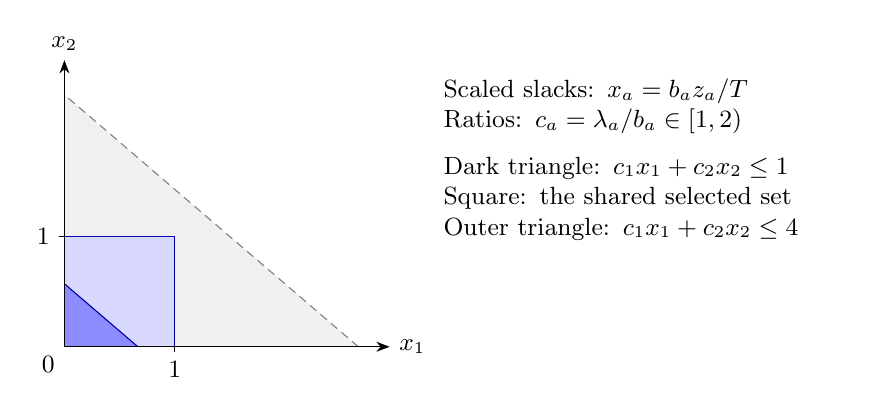
\begin{tikzpicture}[x=1.4cm,y=1.4cm,font=\small,>=Stealth]
\fill[gray!12] (0,0)--({8/3},0)--(0,{16/7})--cycle;
\fill[blue!15] (0,0) rectangle (1,1);
\fill[blue!45] (0,0)--({2/3},0)--(0,{4/7})--cycle;
\draw[gray,densely dashed] ({8/3},0)--(0,{16/7});
\draw[blue!65!black] (0,0) rectangle (1,1);
\draw[blue!65!black] ({2/3},0)--(0,{4/7});
\draw[->] (0,0)--(2.95,0) node[right] {$x_1$};
\draw[->] (0,0)--(0,2.6) node[above] {$x_2$};
\node[below left] at (0,0) {$0$};
\draw (1,0)--(1,-.045) node[below] {$1$};
\draw (0,1)--(-.045,1) node[left] {$1$};
\node[anchor=west,align=left,text width=5.2cm] at (3.35,1.7)
 {Scaled slacks: $x_a=b_a z_a/T$\\
  Ratios: $c_a=\lambda_a/b_a\in[1,2)$\\[2mm]
  Dark triangle: $c_1x_1+c_2x_2\le1$\\
  Square: the shared selected set\\
  Outer triangle: $c_1x_1+c_2x_2\le4$};
\end{tikzpicture}
% Five labels on the axes and five lines in the legend; two extra lines allow for wrapping.
\addtocounter{linenumber}{12}
\caption{The local cap rule in two coordinates, drawn for $c_1=3/2$ and $c_2=7/4$. Nonnegative coordinates put the true $T$-cap inside the unit square. The square is fixed throughout the bin and has deficit below $4T$. With three coordinates the same argument gives $6T$.}
\label{fig:localbox}
\end{figure}

\begin{lemma}[Shared local caps]\label{lem:local}
For every query in this frame and bin,
\[
 \{k\in G_F:h-\ip qk\le T\}\subseteq A_{F,b}
       \subseteq\{k\in G_F:h-\ip qk\le6T\}.
\]
The set contains $v$ and depends only on the frame and bin. All required moment vectors for a query list $Q$ in a fixed frame can be computed in $(p+|Q|)\poly(L,\log n)$ word operations.
\end{lemma}
\begin{proof}
If the sum in~\eqref{eq:nonnegative} is at most $T$, every nonnegative summand is at most $T$, and $b_a z_a\le\lambda_a z_a\le T$. Conversely, a selected key has $\lambda_a z_a<2T$ for each positive coefficient and zero contribution from each zero coefficient. Its total deficit is at most $6T$. At $v$ all three slacks vanish.

There are $O(L)$ possible bins per coefficient, because a positive height-$O(L)$ rational lies between $2^{-O(L)}$ and $2^{O(L)}$. Group the queries by their at most $O(L^3)$ occupied bin triples. For each triple scan $G_F$, test~\eqref{eq:localset}, and add the original-coordinate weights~\eqref{eq:moments}. Store the resulting vector once and let its queries refer to it. The moments never use the transformed slack coordinates.
\end{proof}

\section{The exceptional keys have linear expected total size}\label{sec:sampling}
For a sampled facet $f$, let
$C_f=\{k\in K:f\cdot(k-o)>1\}$ be its conflict list. Since $B_F$ is the union of the three lists in its frame, Lemma~\ref{lem:frames} gives the deterministic bound
\begin{equation}\label{eq:copies}
 \sum_F|B_F|\le9\sum_f|C_f|.
\end{equation}
Unions remove duplicate key identities. Only frames receiving queries create children.

\begin{lemma}[Expected conflicts with fixed anchors]\label{lem:conflicts}
Suppose every four keys of $K$ are affinely independent. Force four fixed keys into a sample and include every other key independently with probability $\pi\in(0,1)$, where $p\pi\ge4$. Then
\[
 \mathbb E\sum_{f\text{ sampled facet}}|C_f|\le32p.
\]
\end{lemma}
\begin{proof}
Consider an oriented triple whose inner halfspace contains the four anchors. Let $b\le3$ of its defining keys be unforced, and let $c$ keys lie strictly outside. It is a sample facet with probability $\pi^b(1-\pi)^c$. Triples with an exterior anchor have probability zero at either sampling rate. Comparing rates $\pi$ and $\pi/2$ gives
\[
 \frac{c\,\pi^b(1-\pi)^c}{(\pi/2)^b(1-\pi/2)^c}
 \le8c e^{-\pi c/2}\le\frac{16}{\pi}.
\]
The half-rate sample is full-dimensional because of its anchors. If it has $V$ hull vertices, it has $2V-4$ facets. Its expected facet count is therefore at most
$2(4+(p-4)\pi/2)-4\le4+p\pi$.
Sum the comparison over the oriented triples. Each sampled facet has exactly one defining triple and orientation, so
\[
 \mathbb E\sum_f|C_f|
 \le(16/\pi)(4+p\pi)\le32p.\qedhere
\]
\end{proof}

For the entire execution fix
\begin{equation}\label{eq:parameters}
 r=2^{\ceil{\sqrt{\ell}}},\qquad s=512\ell r.
\end{equation}
Sample work is polynomial in $r$, while the constant factor in expected key duplication repeats for $O(\log_r n)$ levels. Choosing $\log r=\Theta(\sqrt{\log n})$ balances these two costs.
At a node with $p\le4s$ keys, inspect its pairs directly. Otherwise, use its first four keys as anchors. Choose a dyadic probability
$s/p\le\pi<2s/p<1/2$ and sample the other keys independently. A draw uses at most $O(\log n)$ random bits.

Accept the sample only if it has at most $8s$ keys and every facet conflict list has size at most $p/(4r)$. The checks use the actual lists. Any failure makes this node a direct leaf; no resampling loop is used. General position holds for every current list by Lemma~\ref{lem:preprocess}.

\begin{lemma}[Checked recursive step]\label{lem:step}
On a general-position input, a nonterminal node fails its checks with probability at most $(n+2)^{-100}$. Every accepted child has fewer than $p/r$ keys. Conditional on any earlier history and a fixed general-position input, the expected total number of child-key memberships is at most $288p$. Query lists partition.
\end{lemma}
\begin{proof}
There are fewer than $2p^3$ candidate oriented facets. A triple with more than $p/(4r)$ exterior keys is sampled as a facet with probability at most
$\exp(-\pi p/(4r))\le e^{-128\ell}$.
A union bound controls every heavy facet. For the sample size, the number $Z$ of unforced sampled keys has mean at most $2s$. If the total size exceeds $8s$, then $Z\ge7s$, and
$\Pr[Z\ge7s]\le \mathbb E[2^Z]/2^{7s}\le e^{2s}2^{-7s}\le e^{-2s}$.
These bounds sum to less than $(n+2)^{-100}$.

Each child is a union of three accepted conflict lists, so its size is at most $3p/(4r)<p/r$. Equations~\eqref{eq:copies} and Lemma~\ref{lem:conflicts} bound the expected child mass by $9\cdot32p$. Rejected nodes have no children, which only lowers this unconditional expectation. No conditioning on successful sampling is needed. Assigning each query to one frame makes its destination unique.
\end{proof}

\section{The algorithm and its proof}\label{sec:algorithm}
Precompute each key's integer vector $(\kappa_j^\alpha,\nu_j\kappa_j^\alpha)_{|\alpha|\le g}$. A node owns a key list $K$ and a query list $Q$. A direct leaf computes, for each of its queries, the exact maximum $h$ over $K$ and the moments of $\{k\in K:h-\ip qk\le T\}$. It records this pair $(h,\text{moment vector})$ for the query.

At an accepted node, construct the frames and assign the queries. For each occupied frame, compute the local bin summaries from Lemma~\ref{lem:local}. Each query records its $h=\ip qv$ and a reference to its bin's moment vector. Recurse on $B_F$ with the queries assigned to that frame, unless $B_F$ is empty. All bins of a frame share this one child. All checks precede recording contributions, so a fallback cannot add a contribution twice.

\begin{figure}[t]
\centering
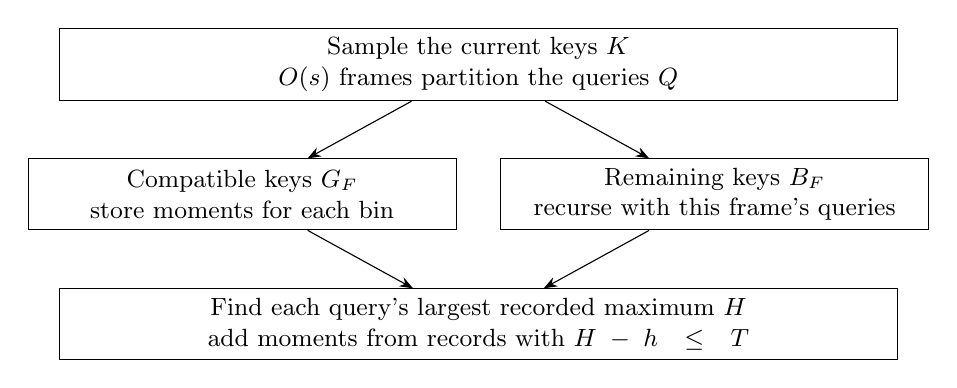
\begin{tikzpicture}[font=\small,>=Stealth,
 box/.style={draw,align=center,text width=5.2cm,minimum height=.9cm}]
\node[box,text width=10.4cm] (root) at (0,0) {Sample the current keys $K$\\$O(s)$ frames partition the queries $Q$};
\node[box] (good) at (-3.0,-1.65) {Compatible keys $G_F$\\store moments for each bin};
\node[box] (bad) at (3.0,-1.65) {Remaining keys $B_F$\\recurse with this frame's queries};
\node[box,text width=10.4cm] (end) at (0,-3.3) {Find each query's largest recorded maximum $H$\\add moments from records with $H-h\le T$};
\draw[->] (root)--(good);
\draw[->] (root)--(bad);
\draw[->] (good)--(end);
\draw[->] (bad)--(end);
\end{tikzpicture}
% Account for all text lines in the diagram, beyond the automatically counted caption.
\addtocounter{linenumber}{10}
\caption{At each node a query uses one frame. Its compatible keys contribute a summary; its remaining keys follow one recursive path. The recorded pieces are disjoint even though other queries may use different pieces.}
\label{fig:recursion}
\end{figure}

\begin{lemma}[Deferred support and final cap]\label{lem:deferred}
For a query, let $(h_t,M_t)$ be its recorded pairs and put $H=\max_t h_t$. Then $H$ is its exact global maximum. The sum of $M_t$ over records with $H-h_t\le T$ is precisely the moment vector of a set satisfying~\eqref{eq:sandwich}.
\end{lemma}
\begin{proof}
The query follows one path. At each nonterminal node its current keys split into $G_F$ and $B_F$, and only the latter continue. These good sets, together with a final leaf if present, partition the original keys. Each piece has exact maximum $h_t$: a good piece contains its sampled support vertex, and a leaf finds its maximum directly. Every local selected set contains that maximiser. Hence $\max_t h_t=H$ is the global maximum.

A key with global deficit at most $T$ lies in one piece and satisfies
\[
 0\le H-h_t\le H-\ip qk\le T,\qquad
 0\le h_t-\ip qk\le T.
\]
Its record is kept, and it is selected by Lemma~\ref{lem:local} or the leaf rule. Conversely, every selected key in a kept record has global deficit at most $T+6T=7T$. The pieces are disjoint, so summing their moments counts each selected key once.
\end{proof}

\begin{proof}[Proof of Theorem~\ref{thm:main}]
The two numerical lemmas and Lemma~\ref{lem:deferred} prove the error guarantee for every completed execution. It remains to bound the word operations, including unsuccessful checks.

All accepted children shrink their key lists by a factor greater than $r$, and rejected nodes stop. Thus every execution terminates within $d_0=1+\ceil{\log_r n}=O(\sqrt{\log n})$ levels. At every depth the query lists are disjoint, so their total size is at most $n$. Lemma~\ref{lem:step}, applied conditionally at each node, gives expected total key-list size at most $288^j n$ at depth $j$.

The bounded sample, its hull and frames, all conflict tests, and the local summaries cost
$(p+|Q|)\poly(s,\log n)$ at a node. A small direct leaf costs at most $4s|Q|\poly(\log n)$. At a larger node, direct inspection after a failed check adds at most $p|Q|\poly(\log n)$, with conditional probability at most $(n+2)^{-100}$. Its expected cost is bounded by $(n+2)^{-99}p\poly(\log n)$. Summing these bounds over depths yields
\[
 n\,(d_0+1)\,288^{d_0}\poly(s,\log n)
       =n\,2^{O(\sqrt{\log n})}.
\]

For the bit bound, a sample centre averages four original preprocessed keys. Facet normals and frame coefficients solve fixed-size rational systems in those keys and original queries. Their heights are $O(\log n)$, independently of the depth. Children retain original coordinates. The moment additions and final exact reconstruction have $O(\log^2 n)$-bit intermediates by Lemma~\ref{lem:moments}. All displayed costs are therefore word costs.

Finally choose a fixed sufficiently large integer $C$ so that
$A(n)=2^{\ell+C\ceil{\sqrt{\ell}}}\ell^C$
dominates the expected operation count for every $n\ge2$. Its integer counter has $O(\log n)$ bits. Stop after $3A(n)$ operations and return zero if unfinished. Markov's inequality makes this event have probability at most $1/3$, proving the worst-case statement. The fixed finite algorithms above determine an absolute such $C$, so the algorithm is uniform.
\end{proof}

\section{Scope and remaining questions}\label{sec:scope}
The proof uses the linear face complexity of three-dimensional hulls twice: to bound expected facet conflicts and to bound the number of frames. A fan triangulation from one polar vertex can repeat a facet in many frames. Alternating ears prevents this duplication and gives the sharper $n\,2^{O(\sqrt{\log n})}$ bound.

The upper bound is asymptotic. Its sample parameter and moment degree are chosen for a simple proof, and their constants are large. The finite checkers in the supplementary material exercise the geometric partition, exact moment identities, and sampling estimates. They use exact arithmetic on small inputs and do not measure running time. Higher fixed dimensions require a different analysis, because sampled hulls can have superlinear face complexity.

\subsection*{Acknowledgements}
GPT-6 Astra Pro and Claude Opus 5.5 assisted with the proofs, which the author checked line by line.

\bibliographystyle{plainurl}
\bibliography{references}
\clearpage
\appendix

\section{Finite input rounding and general position}\label{app:preprocess}
\begin{proof}[Proof of Lemma~\ref{lem:preprocess}]
Let $R$ be the least power of two at least $16384n^{24}$. Round every query coordinate, key coordinate, and value to the nearest multiple of $1/R$, breaking ties consistently. Because $B=n^{10}$ and $1$ belong to the grid, rounding stays within the original magnitude intervals. Each coordinate changes by at most $1/R$, and each score by at most $9B/R$.

For $p=\operatorname{softmax}(a)$, differentiation in direction $z$ gives
\[
 (D\operatorname{softmax}(a)z)_j
   =p_j\left(z_j-\sum_t p_tz_t\right),\qquad
 \norm{D\operatorname{softmax}(a)z}_1\le2\norm z_\infty.
\]
Integration along a segment and $|v_j|\le1$ bound the output change, including the rounded values, by $(18B+1)/R<n^{-10}/128$.

Use the global key identities $j=1,\ldots,n$ to define
\[
 t_j=j/2^\ell,\qquad m_j=(t_j,t_j^2,t_j^3),\qquad
 \theta=2^{-128\ell},\qquad k'_j=(1-\theta)k_j+\theta m_j.
\]
Here $0<t_j<1$, so the magnitude bound is preserved. Each key coordinate moves by at most $2B\theta$, and each score by at most $6B^2\theta$. The same derivative estimate bounds the attention-output change by $12B^2\theta<n^{-10}/128$. Together the two errors are below the lemma's stated budget.

Since $2^\ell<2(n+2)\le4n$, we have $2^{3\ell}<64n^3\le R$. Both are powers of two. Thus every $m_j$ belongs to $R^{-1}\Z^3$, and all resulting coordinates and values belong to the grid with denominator $D=R\,2^{128\ell}$. Its bit length is $O(\log n)$.

It remains to prove general position. Fix four distinct identities $j_0,j_1,j_2,j_3$ and put
\[
 a_i=k_{j_i}-k_{j_0},\qquad b_i=m_{j_i}-m_{j_0},\qquad
 w=\frac{\theta}{1-\theta}\quad(i=1,2,3).
\]
Their perturbed affine determinant equals $(1-\theta)^3 P(w)$, where
\[
 P(w)=\det(a_1+wb_1,a_2+wb_2,a_3+wb_3)
       =c_0+c_1w+c_2w^2+c_3w^3.
\]
The cubic coefficient is the nonzero Vandermonde determinant of the four distinct moment-curve points. Every coefficient belongs to $R^{-3}\Z$. Moreover, the coordinate bounds $|a_{ia}|\le2B$ and $|b_{ia}|\le1$, together with the six-term determinant expansion, give
\[
 |c_1|\le72B^2,\qquad |c_2|\le36B,\qquad |c_3|\le6,
 \qquad |c_1|+|c_2|+|c_3|\le114B^2.
\]
Let $c_h$ be the first nonzero coefficient. Then $|c_h|\ge R^{-3}$. Because $0<w<1$, the higher-degree terms after dividing by $w^h$ have total absolute value at most $114B^2w$. On the other hand,
\[
 R^3\,114B^2w
 <2^{42+72\ell}\,2^7\,2^{20\ell}\,2^{1-128\ell}
 =2^{50-36\ell}<1,
\]
using $R\le2^{14+24\ell}$ and $\ell\ge2$. These terms cannot cancel $c_h$. Hence $P(w)\ne0$, proving general position for every quadruple.

The construction separates repeated original positions by their identities. It uses a fixed number of $O(\log n)$-bit rational operations per key; descendants retain the resulting coordinates and global identities. For fewer than four keys the condition is vacuous and the algorithm uses direct inspection.
\end{proof}

\section{Exact reconstruction from integer moments}\label{app:numerics}
\begin{proof}[Proof of Lemma~\ref{lem:moments}]
Let $P_g(z)=\sum_{r=0}^g z^r/r!$. On $-7T\le z\le0$, Taylor's theorem gives a remainder at most $(7T)^{g+1}/(g+1)!$: the derivative at its intermediate point is at most one. Since $e<3$, $r!\ge(r/e)^r$, and $g=64T$,
\[
 |e^z-P_g(z)|
 \le\left(\frac{21T}{g+1}\right)^{g+1}
 \le2^{-(g+1)}\le2^{-T}.
\]
An omitted key also has exponential weight at most $e^{-T}\le2^{-T}$. For a fixed row write
\[
 D_*=\sum_j e^{-\Delta_j},\quad N_*=\sum_j e^{-\Delta_j}v_j,\qquad
 \widehat D=\sum_{j\in A}P_g(-\Delta_j),\quad
 \widehat N=\sum_{j\in A}P_g(-\Delta_j)v_j.
\]
The sandwich includes a maximiser, so $D_*\ge1$ and $|N_*|\le D_*$. Each of the two sums changes by at most $2n2^{-T}$. Hence $\widehat D>0$ and
\begin{equation}\label{eq:ratio}
 \left|\frac{\widehat N}{\widehat D}-\frac{N_*}{D_*}\right|
 \le\frac{4n2^{-T}}{1-2n2^{-T}}
 \le8n2^{-T}<n^{-10}/32.
\end{equation}
Here $2^{-T}\le(n+2)^{-32}$.

For the integer calculation, put $J=D^2H\in\Z$, where $H$ is the exact row maximum. Define
\begin{equation}\label{eq:integercoef}
 F_0=1,\qquad F_s=sD^2F_{s-1}+(-J)^s,\qquad
 C_\alpha=\binom{g}{\alpha_1,\alpha_2,\alpha_3,g-|\alpha|}
                  \xi^\alpha F_{g-|\alpha|}.
\end{equation}
Then
\begin{equation}\label{eq:integeridentity}
 g!D^{2g}P_g\!\left(\frac{\ip{\xi}{\kappa}-J}{D^2}\right)
       =\sum_{|\alpha|\le g}C_\alpha\kappa^\alpha.
\end{equation}
Indeed $F_s=\sum_{r=0}^s(s!/r!)(-J)^rD^{2(s-r)}$ by induction. Expanding the Taylor polynomial by the multinomial theorem and collecting each $\kappa^\alpha$ gives exactly~\eqref{eq:integeridentity}.

Contract the right side with the unweighted moments to obtain $Z$, and with the $\nu$-weighted moments to obtain $W$. Then $\widehat N/\widehat D=W/(DZ)$ and $Z>0$. No approximate arithmetic has yet occurred.

The bounds $|\xi_a|,|\kappa_{ja}|\le DB$, $|\nu_j|\le D$, and $|J|\le3D^2B^2$ give
\[
 |F_s|\le s!(s+1)\max\{D^2,|J|\}^s.
\]
Every multinomial coefficient is at most $4^g$. Thus the bit length of every term, weight sum, coefficient, and intermediate contraction is
\[
 O\bigl(\log n+g(\log D+\log(B+1)+\log(g+2))\bigr)
       =O(\log^2 n).
\]
This bounds absolute magnitudes before cancellation. There are polynomially many coefficients in $g$, and elementary integer arithmetic suffices. Round $W/(DZ)$ to the nearest multiple of $2^{-16\ell}$. The extra error is at most $2^{-16\ell-1}<n^{-10}/128$. Together with~\eqref{eq:ratio} this proves the lemma.
\end{proof}

\section{Constructing and checking the small-hull frames}\label{app:frames}
All hull constructions in the algorithm have at most $8s$ points. Polynomial work in $s$ contributes only $2^{O(\sqrt{\log n})}$, so no sophisticated polytope query structure is required.

\paragraph*{Hull and centre.}
At a nonterminal node the first four current keys are affinely independent by Lemma~\ref{lem:preprocess}. They are the forced anchors, and their centroid $o$ lies strictly inside the sampled hull. Abort to a direct leaf if the sample exceeds its size cap. Every sampled quadruple is affinely independent, so the remaining hull construction uses bounded loops on nondegenerate data.

For each sampled triple, form its plane by a cross product and test all other sampled points. It is a facet precisely when they lie strictly on one side. Orient its normal $a$ outward, put $b=a\cdot(v-o)>0$ for a vertex $v$ of the triple, and store $f=a/b$. Vertex, edge, and facet incidences follow from the triples. Every facet is triangular, every edge is in two facets, and the facets incident to a vertex have a cyclic order given by sharing edges through that vertex.

\paragraph*{Why the normal polygon covers the queries.}
At a hull vertex $v$ the cone of its incident outward facet normals is its normal cone. One direct argument is as follows. This finitely generated cone is closed: its generators lie in the affine plane $f\cdot(v-o)=1$, so a bounded sequence in the cone has bounded conic coefficients. If a maximising query $q$ were outside it, project $q$ onto the closed cone. The displacement $d$ from that projection satisfies $f\cdot d\le0$ for every incident facet and $q\cdot d>0$. For sufficiently small $\eta>0$, $v+\eta d$ still satisfies the incident inequalities and all nonincident inequalities, which have positive slack at $v$. This contradicts maximality of $v$.

Intersect this cone with $u\cdot(v-o)=1$. The result is the convex hull of the incident normal vectors. Every one is a vertex of that polygon: if one were a convex combination of the others, its facet inequality would be implied by the others, contradicting a point in the relative interior of that facet. The incident normals span $\R^3$, since otherwise $v\pm\eta d$ would both remain feasible for a small displacement orthogonal to them, contradicting that $v$ is a vertex. Thus the polygon is two-dimensional, and each of its triangles has three linearly independent vectors.

\paragraph*{Bounded-degree triangulation.}
For cyclic vertices $a_1,\ldots,a_h$, successively remove $a_1,a_h,a_2,a_{h-1},\ldots$, recording the ear at each removal, and include the final remaining triangle. Convexity makes every recorded triangle a valid ear. A vertex first appears when it or its neighbour becomes an end of the remaining chain; it then appears in at most the next opposite-end ear and its own ear. The two end vertices of the final triangle have the same bound. Thus every vertex appears in at most three triangles, also for $h=3$.

The frames are precisely these triangles, with their primal vertex $v$. A triangular facet is incident to three vertices, so its normal is used at most nine times. This is a bound over all frames of the sample, including those that receive no queries.

\paragraph*{Assignments, checks, and heights.}
Scan the frames for each query, solving $q=\sum_a\lambda_af_a$ by Cramer's rule, and choose the first solution with all coefficients nonnegative. The preceding argument guarantees one exists. Cone boundaries need no perturbation; zero coefficients receive their own dyadic-bin symbol. If a construction or assignment fails a check, discard the node's temporary work and use direct inspection before recording any contribution.

Construct each conflict list by checking its facet inequality against every current key. Reject the sample if any list exceeds $p/(4r)$. For a frame, form the union of its three lists by key identity. Its complement is $G_F$, and this checked partition is what the recursion uses. Keys with equality satisfy the facet inequality and are compatible.

All facet planes use three original preprocessed keys, and the centre uses four. Frame coefficients use three such normals and one original query. There is a fixed bound on the number of rational operations in each expression, so every height is $O(\log n)$. No expression contains a coordinate constructed by a parent node. Dyadic-bin endpoints are found by comparisons with powers of two and have the same height bound. Local moment vectors contain original key powers on the global grid; they require no common denominator across different frames.

\typeout{SOCG-MAIN-LINES: \thesocglastlinecounter}
\end{document}
